\section{Results}

Let's explore the test phase and see the results in detail. Initially we ran debug tests on our personal PCs in order to easily modify the code, these starting tests and the tests utilized to determine the right value for the many defined constants(altogether the vast majority of the tests done) are not shown here. 

All the tests shown below were performed on a single more powerful machine that has enabled us to work with much larger data in less time. The machine used is composed of two Xeon processors for a total of 16 cores 2.80 Ghz and 48 Gb of RAM.

The tests were performed on a growing number of scans, each containing a maximum of 50 lines from which we extracted the words that represent the states. For each set of scans we present three possible distances calculation: only LCS, only L1 (Euclidean distance) and LCS and L1 combined together through the formula presented in Section 5.

\vspace{3mm}

The data fields for each test are defined as follows:
\begin{itemize}
\item \textbf{Number of scans}: the number of scans that were utilized in the test.
\item \textbf{Estimated words}: the number of words estimated on the basis of the number of scans(50x).
\item\textbf{Extracted words}: the number of words actually mined and processed, as well as the corresponding percentage.
\item \textbf{Number of clusters}: the number of clusters created in process.
\item \textbf{Features extraction time}: the time, in seconds, required for features extraction from the words.
\item \textbf{Evaluating distances time}: the time, in seconds, required to generate the similarity matrix with the distances between all the words extracted.
\item \textbf{Clustering time}: the time, in seconds, required for the creation of clusters.
\item \textbf{Running time}: the total execution time, in seconds.
\item \textbf{Correct clusters}: the number of clusters with absolute precision, therefore containing only words equal to each other.
\item \textbf{Correct elements}: the number of words within the Correct clusters and their corresponding percentage respect to all the elements.
\item \textbf{Average precision}: the accuracy of the results, the average accuracy of clusters.
$$Precision_{average} = \frac{\sum_i P_i}{N_c}$$
where $P_i$ is the precision of cluster $i$ and $N_c$ is the number of clusters. 
\item \textbf{Precision}: the accuracy of the results, the average accuracy of individual clusters weighted with the number of words.
$$Precision = \frac{\sum_i P_i * n_i}{N_w}$$
where $P_i$ is the precision of cluster $i$, $n_i$ is the number of words in cluster $i$ and $N_w$ is the number of words. 
\end{itemize}

In the next table we're going to show the main results of the tests. 

\begin{table}[!htbp]
\centering
\footnotesize
\begin{tabular}{|l | c | c | c | c | c |} 
 \hline 
 & \multicolumn{1}{p{2cm}|}{\centering\bfseries Estimated \\ words}&  \multicolumn{1}{p{2cm}|}{\centering\bfseries Extracted \\ words} & \multicolumn{1}{p{2cm}|}{\centering\bfseries Number of \\ clusters} & \multicolumn{1}{p{2cm}|}{\centering\bfseries Running \\ time (s)} & \multicolumn{1}{p{2cm}|}{\centering\bfseries Precision \\ (\%)} \\ [0.5ex] 
 \hline\hline
%% label & estimated words & extracted words & clusters & time & precision %%
16 scans (L1) & 800 & 550 & 55 & 15.52 & 58.00\\ 
16 scans (LCS) & 800 & 550 & 71 & 44.39 & 60.00\\ 
16 scans (LCS and L1) & 800 & 550 & 66 & 47.41 & 62.91\\ 
32 scans (L1) & 1600 & 800 & 67 & 38.58 & 52.87\\ 
32 scans (LCS) & 1600 & 800 & 92 & 94.54 & 55.50\\ 
32 scans (LCS and L1) & 1600 & 800 & 86 & 112.90 & 56.25\\ 
75 scans (L1) & 3750 & 2350 & 173 & 221.03 & 63.65\\ 
75 scans (LCS) & 3750 & 2350 & 189 & 1169.72 & 67.49\\ 
75 scans (LCS and L1) & 3750 & 2350 & 199 & 1203.28 & 71.16\\ 
130 scans (L1) & 6500 & 5050 & 425 & 5444.43 & 71.12\\ 
130 scans (LCS) & 6500 & 5050 & 441 & 5629.71 & 74.41\\ 
130 scans (LCS and L1) & 6500 & 5050 & 463 & 6729.62 & 77.94\\ 
500 scans (L1) & 25000 & 18146 & 3957 & 85545.11 & 77.89\\ 
500 scans (LCS) & 25000 & 18146 & 3316 &  76324.63 & 81.22\\ 
500 scans (LCS and L1) & 25000 & 18146 & 3941 & 138309.85\tablefootnote{During this test, the machine used was concurrently executing other tasks creating a bottleneck in the memory used.} & 82.14\\ 
 \hline
\end{tabular}
\caption{Main results}
\label{table:1}
\end{table}

As we can see in Table \ref{table:1} the number of extracted words is much less than the estimated number of words. This is mainly due to the fact that not all census tables are filled in full: in some cases there are only a few lines or it has not been filled in the status column. In other cases the error is due to a difficulty in removing the word from the scan due to a wrong interpretation of the rows or the columns.

As we can see in Table \ref{table:prec} and in Figure \ref{fig:precision} the accuracy of the cluster grows with the amount of words extracted. This phenomenon is due to the fact that Affinity Propagation works best with a large number of available data: the greater the number of words, the greater the chances of finding words similar between them, and then combine them within a single cluster.

\begin{table}[!htbp]
\centering
\footnotesize
\begin{tabular}{|l | c | c |} 
 \hline 
 &\multicolumn{1}{p{2cm}|}{\centering\bfseries Average \\ precision (\%)} & \multicolumn{1}{p{2cm}|}{\centering\bfseries Precision \\ (\%)} \\ [0.5ex] 
 \hline\hline
%% label & estimated words & extracted words & clusters & time & precision %%
16 scans (L1) & 65.06 & 58.00\\ 
16 scans (LCS) & 76.56 & 60.00\\ 
16 scans (LCS and L1) & 74.37 & 62.91\\ 
32 scans (L1) & 59.85 & 52.87\\ 
32 scans (LCS) & 72.97 & 55.50\\ 
32 scans (LCS and L1) & 70.19 & 56.25\\ 
75 scans (L1) & 69.03 & 63.65\\ 
75 scans (LCS) & 75.09 & 67.49\\ 
75 scans (LCS and L1) & 78.01 & 71.16\\ 
130 scans (L1) & 76.66 & 71.12\\ 
130 scans (LCS) & 82.11 & 74.41\\ 
130 scans (LCS and L1) & 84.87 & 77.94\\ 
500 scans (L1) & 90.66 & 77.89\\ 
500 scans (LCS) & 91.02 & 81.22\\ 
500 scans (LCS and L1) & 92.27 & 82.14\\ 
 \hline
\end{tabular}
\caption{Precision}
\label{table:prec}
\end{table}

\begin{figure}[!htbp]
\centering
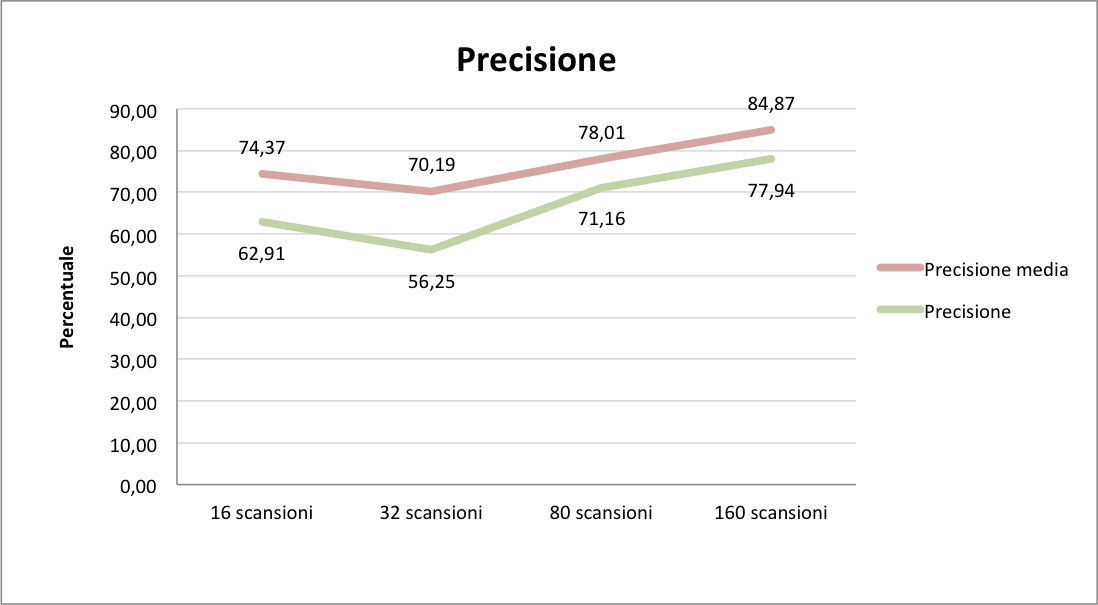
\includegraphics[width=0.7\textwidth]{images/precisione.png}
\caption{Clustering precision based on number of scans}
\label{fig:precision}
\end{figure}

Now we're going to focus our attention to time. The running time is divided mainly into three distinct phases: time for the extraction of features, time for the creation of similarity matrix (calculation of distances) and clustering.

\begin{table}[!htbp]
\centering
\footnotesize
\begin{tabular}{|l | c | c | c | c |} 
 \hline 
 & \multicolumn{1}{p{2cm}|}{\centering\bfseries Features extraction\\time (s)}&  \multicolumn{1}{p{2cm}|}{\centering\bfseries Evaluating distances\\time (s)} & \multicolumn{1}{p{2cm}|}{\centering\bfseries Clustering\\ time (s)} & \multicolumn{1}{p{2cm}|}{\centering\bfseries Total (s)} \\ [0.5ex] 
 \hline\hline
%% label & features & distances & clusters & total %%
16 scans (L1) & 6.81 & 5.02 & 3.69 & 15.52\\ 
16 scans (LCS) & 6.84 & 34.40 & 3.15 & 44.39\\ 
16 scans (LCS and L1) & 6.84 & 37.32 & 2.85 & 47.41\\ 
32 scans (L1) & 11.54 & 7.22 & 19.82 & 38.58\\ 
32 scans (LCS) & 11.27 & 74.72 & 8.55 & 94.54\\ 
32 scans (LCS and L1) & 11.34 & 89.96 & 11.60 & 112.90\\ 
75 scans (L1) & 33.65 & 69.00 & 118.38 & 221.03\\ 
75 scans (LCS) & 35.13 & 1002.63 & 131.96 & 1169.72\\ 
75 scans (LCS and L1) & 34.70 & 1070.92 & 97.66 & 1203.28\\ 
130 scans (L1) & 70.80 & 313.70 & 5059.93 & 5444.43\\ 
130 scans (LCS) & 68.17 & 4353.85 & 1207.69 & 5629.71\\ 
130 scans (LCS and L1) & 73.10 & 5608.82 & 1047.70 & 6729.62\\ 
500 scans (L1) & 289.33 & 4482.02 & 80773.76 & 85545.11 \\ 
500 scans (LCS) & 323.66 & 57699.51 & 18301.46 & 76324.63\\ 
500 scans (LCS and L1) & 403.41 & 61424.57 & 76481.87 & 138309.85\\ 
 \hline
\end{tabular}
\caption{Running time}
\label{table:2}
\end{table}

As we can see in Table \ref{table:2} the computational time is mainly due to the construction phase of similarity matrix, so the calculation of distances. This occurs especially in calculating LCS distance due to the fact that structural strings of words are very long and the cost of the algorithm is $O(nm)$, with $n$ and $m$ the lengths of the two strings.

Structural long strings characterize better the word (and therefore make more accurate clustering), but involve a longer calculation time.

\begin{figure}[!htbp]
\centering
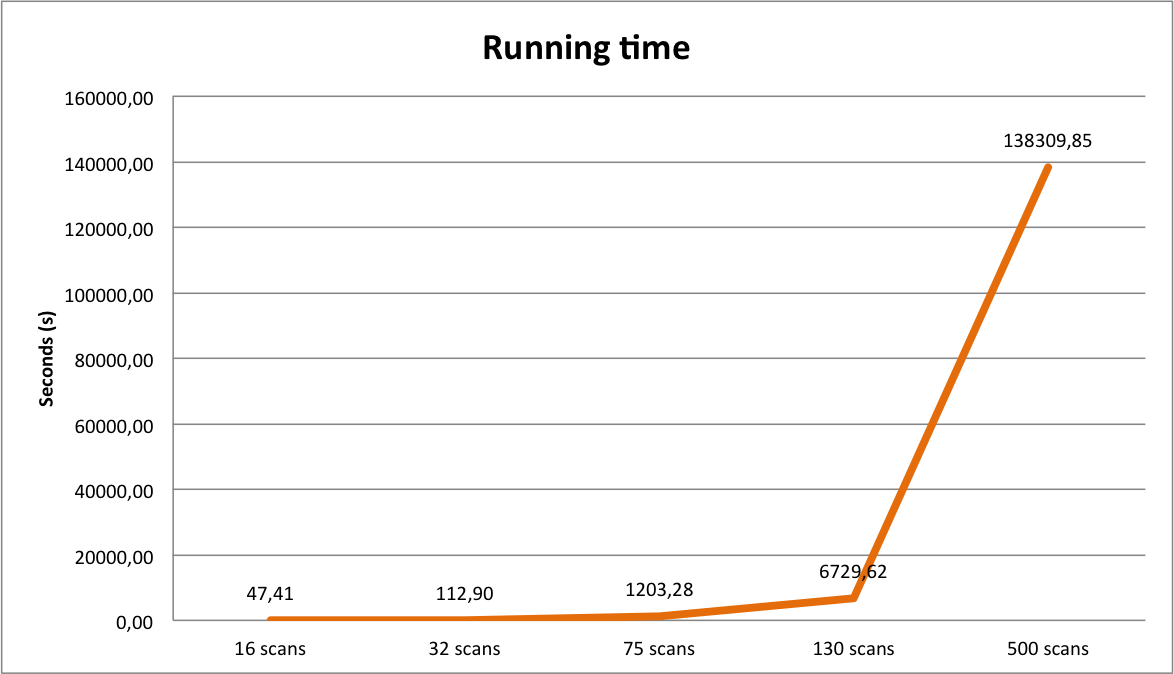
\includegraphics[width=0.7\textwidth]{images/esecuzione}
\caption{Running time on number of scans}
\label{fig:time}
\end{figure}

A parameter to evaluate the goodness of the newly formed clusters can be the number of clusters that have a maximum precision, which contain all similar elements between them and properly classified. This parameter is indicative as it can still exist cases of \emph{false negatives} (words properly classified but labelled incorrectly) that then cut out the entire cluster.

In the following table are collected the number of clusters that respect the above described property and the number of items that they contain. 

\begin{table}[!htbp]
\centering
\footnotesize
\begin{tabular}{|l | c | c | c | c |} 
 \hline 
 & \multicolumn{1}{p{2cm}|}{\centering\bfseries Correct\\ clusters}&  \multicolumn{1}{p{2cm}|}{\centering\bfseries Correct\\words} & \multicolumn{1}{p{2cm}|}{\centering\bfseries Percentage\\of words (\%)} & \multicolumn{1}{p{2cm}|}{\centering\bfseries Average words\\for cluster} \\ [0.5ex] 
 \hline\hline
%% label & clusters & words & percentage %%
16 scans (L1) & 12 & 18 & 3.27 &  1.50\\ 
16 scans (LCS) & 33 & 44 & 8.00 &1.33\\ 
16 scans (LCS and L1) & 25 & 45 & 8.18 & 1.80\\ 
32 scans (L1) & 11 & 11 & 1.38 & 1.00\\ 
32 scans (LCS) & 39 & 48 & 6.00 &1.23\\ 
32 scans (LCS and L1) & 32 & 43 & 5.38 & 1.34\\ 
75 scans (L1) & 39 & 172 & 7.32 & 4.41\\ 
75 scans (LCS) & 78 & 265 & 11.28 & 3.40\\ 
75 scans (LCS and L1) & 77 & 316 & 13.45 & 4.10\\ 
130 scans (L1) & 138 & 651 & 12.89 & 4.72\\ 
130 scans (LCS) & 208 & 713 & 14.12 &  3.43\\ 
130 scans (LCS and L1) & 215 & 860 & 17.03 & 4.00\\ 
500 scans (L1) & 2854 & 7354 & 40.53 & 2.58\\ 
500 scans (LCS) & 2902 & 7423 & 40.91 & 2.56\\ 
500 scans (LCS and L1) & 3020 & 7616 & 41.97 & 2.52\\ 
 \hline
\end{tabular}
\caption{Correct clusters}
\label{table:3}
\end{table}
